\input{header}

\AtBeginSubsection[]
{
	\begin{frame}<beamer>
		\frametitle{Outline}
		\tableofcontents[current,currentsubsection]
	\end{frame}
}

\begin{document}

\begin{frame}[allowframebreaks] \frametitle{Turing-recognizable}
  \begin{itemize}
\item A language if Turing-recognizable if it is recognized by a TM
\item For a Turing machine, there are three possible outcomes
  \begin{center}
accept, reject, loop
\end{center}
\item If an input fails: reject or loop

\item [] This is difficult to decide
\item We prefer a TM that never loops

\item [] Deciders: only accept or reject
\item A language is Turing-decidable if some TM decides it
\item In Chapter 4 we will discuss decidable languages
  
\end{itemize}\end{frame} \begin{frame}[allowframebreaks] \frametitle{Example 3.9}
  \begin{itemize}
  \item Consider the following language
    \begin{equation*}
    \{w\# w\mid w\in \{0,1\}^*\}
  \end{equation*}

\item Fig 3.10  
 
\end{itemize}

\begin{tikzpicture}
\node[state,initial left] (q_1) {$q_1$};
\node[state] (q_2) [below left of=q_1,yshift=0.7cm,xshift=-2.5cm] {$q_2$};
\node[state] (q_8) [below of=q_1,yshift=1cm] {$q_8$};
\node[state] (q_3) [below right of=q_1,yshift=0.7cm,xshift=2.5cm] {$q_3$};
\node[state] (q_4) [below of=q_2,yshift=1.2cm] {$q_4$};
\node[state] (q_a) [below of=q_8,yshift=1.2cm] {$q_a$};
\node[state] (q_5) [below of=q_3,yshift=1.2cm] {$q_5$};
\node[state] (q_6) [below of=q_a,yshift=1.3cm] {$q_6$};
\node[state] (q_7) [left of=q_6,xshift=0cm] {$q_7$};
 \path 
 (q_1) edge[above]  node {$0 \rightarrow$ x, R} (q_2)
 (q_1) edge[right]  node {$\# \rightarrow$ R} (q_8)
 (q_1) edge[above]  node {$1 \rightarrow$ x, R} (q_3) 
 (q_2) edge[loop above]  node {0,1 $ \rightarrow $ R} (q_2)
 (q_2) edge[right]  node {$\# \rightarrow$ R} (q_4)  
 (q_8) edge[loop right]  node {x $ \rightarrow $ R} (q_8)
 (q_8) edge[right]  node { $\sqcup \rightarrow $ R} (q_a)
 (q_3) edge[loop above]  node {0,1 $ \rightarrow $ R} (q_3)
 (q_3) edge[left]  node {$\# \rightarrow$ R} (q_5)
 (q_4) edge[loop below]  node {x $\rightarrow$ R} (q_4)
 (q_4) edge[above]  node {0 $\rightarrow$ x, L} (q_6)
 (q_5) edge[loop below]  node {x $\rightarrow$ R} (q_5)
 (q_5) edge[above]  node {1 $\rightarrow$ x, L} (q_6)
 (q_6) edge[loop right]  node {0, 1,  x $\rightarrow$ L} (q_6)
 (q_6) edge[below]  node {$\# \rightarrow$ L} (q_7)
 (q_7) edge[loop left]  node {0, 1 $\rightarrow$ L} (q_7)
 (q_7) edge[bend right=15, left]  node {x $\rightarrow$ R} (q_1)    
;
\end{tikzpicture}

\begin{itemize}
\item Links to $q_r$ not shown
\item Simulate $01\#01$

\begin{center}
\begin{tabular}{llll}
  $q_1 0 1 \# 01$ & $x q_2 1 \# 01$ & $x1 q_2 \# 01$ & $x1\# q_4 01$
  \\
  $x1 q_6 \# x 1$ & $x q_7 1 \# x 1$ & $ q_7 x 1 \# x 1$ & $x q_1 1 \# x 1$
  \\
  $xx q_3 \# x 1$ & $xx \# q_5 x 1$ & $xx \# x q_5 1$ & $xx \# q_6 xx$ \\
  $xx q_6 \# xx$ & $x q_7 x \# xx$ & $xx q_1 \# xx$ & $xx \# q_8 xx$ \\
 $xx \# xx q_8 \sqcup$ &  $xx \# xx \sqcup q_a$ &&
\end{tabular}
\end{center}
  
\end{itemize}

\end{frame}

\begin{frame}[allowframebreaks] \frametitle{Example 3.11}
  \begin{itemize}
\item $C=\{a^i b^j c^k\mid i\times j=k, i,j,k \geq 1\}$
\item Procedure
  \begin{enumerate}
  \item check if the input is $a^+ b^+ c^+$
  \item back to start
  \item fix $a$, for each $b$, cancel $c$
  \item store $b$ back, cancel one $a$, goto step 3
  \end{enumerate}
\item Too complicated to draw state diagram
\item But one may wonder if TM can really do the above procedure
\item Here are more details
\item Step 1 can be done by a DFA (as DFA is a special case of TM)
\item Step 2 can be done by using a special symbol in the beginning
\item Step 3 is similar to the procedure of handling $w\#w$
\item [] Now we see the concept of subroutines
\end{itemize}\end{frame} \begin{frame}[allowframebreaks] \frametitle{Example 3.12}
  \begin{itemize}
\item $E=\{\#x_1\# x_2 \cdots \# x_l\mid x_i \in 
\{0,1\}^*, x_i \neq x_j\}$
\item Idea: sequentially compare every pair

  \begin{equation*}
    \begin{split}
& x_1 x_2, x_1 x_3, \ldots, x_1 x_l \\
& x_2 x_3, \ldots, x_2 x_l \\
& x_{l-1} x_l
\end{split}
\end{equation*}
\item Very rough $\Rightarrow$ more details

\item [] For $x_i, x_j$ mark \#'s of both strings
by $\dot{\#}$

\item [] $\dot{\#}x_1\#x_2 \dot{\#}x_3$: $x_1$ and $x_3$
being compared
\item Compare $x_i$ and $x_j$:

\item [] Can use a TM similar to that for $w \# w$

\item We can copy $x_1, x_2$ to the end
  and do the comparison there
  
% $\dot{\#}x_1\dot{\#}x_2 \# x_3 \hat{\#}x_1
% \hat{\#}x_2$

% $\dot{\#}x\ldots x\dot{\#}x\ldots x \ldots  \# x_3 \hat{\#}x_1
% \hat{\#}x_2$


% Copy $x_1,x_2$ back

% remove $\hat{\#}x_1
% \hat{\#}x_2$

\end{itemize}\end{frame}

\begin{frame}[allowframebreaks] \frametitle{Variants of TM}
  \begin{itemize}
\item We discuss some variants that have the same power

\item
  The robustness of a type of machines means that its reasonable
variants have the same 
power

\item
  [] Not a strict definition though

\item Example
  \begin{equation*}
\delta: Q \times \Gamma\rightarrow Q \times \Gamma 
\times \{L, R, S\}
\end{equation*}
\item
  [] $S$: stay at the same position

\item
  It's equivalent to TM because $S$ can
  be implemented by $L$ \& $R$ moves:
  \begin{equation*}
      q_1,a \rightarrow q_2,b, S
    \end{equation*}
    can be replaced by several rules
    \begin{equation*}
q_1,a \rightarrow q_3, \quad b,R \rightarrow
q_2, ?, L, \forall ? in \Gamma 
\end{equation*}
\end{itemize}
\end{frame}

\begin{frame}[allowframebreaks] \frametitle{Multi-tape TM}
  \begin{itemize}
\item several tapes
\item input: put into tape 1

\item
  [] others: blank
\item transition is applied on all tapes simultaneously
  \begin{eqnarray*}
&& \delta: Q \times \Gamma^k \rightarrow 
Q \times \Gamma^k \times \{L, S, R\}^k     \\
&& \delta(q_i, a_1, \ldots, a_k)
= (q_j, b_1, \ldots, b_k, L, R, \ldots, L),
  \end{eqnarray*}
where $k$ is the number of tapes
\item Looks more powerful but equivalent


\end{itemize}\end{frame} \begin{frame}[allowframebreaks] \frametitle{Example}

  \begin{itemize}
\item Job: given $w = 0^{2n}, n \geq 0$
$\Rightarrow$ generate $ww$ in the end

\item
  [] Note that we also need to check if $|w|$ is even

\item State diagram

  \end{itemize}

\begin{tikzpicture}
  \node[state,initial below] (q_0) {$q_0$};
  \node[state,right of=q_0,xshift=-0.3cm] (q_1) {$q_1$};
  \node[state,right of=q_1,xshift=-0.3cm] (q_2) {$q_2$};
  \node[state,right of=q_2,xshift=-0.5cm] (q_3) {$q_3$};
  \node[state,right of=q_3,xshift=-0.3cm] (q_4) {$q_4$};
  \node[state,below of=q_4,yshift=0.5cm] (q_a) {$q_a$};
  \path (q_0) edge[above] node{
    \begin{tabular}{l}
      $0 \rightarrow$ R\\
      $\sqcup \rightarrow$ R      
    \end{tabular}
  } (q_1);
  \path (q_1) edge[loop below] node{
    \begin{tabular}{l}
      $0 \rightarrow$ R\\
      $\sqcup \rightarrow 0,$ R      
    \end{tabular}
  } (q_1);
  \path (q_1) edge[above] node{
    \begin{tabular}{l}
      $\sqcup \rightarrow$ L\\
      $\sqcup \rightarrow$ L      
    \end{tabular}
    } (q_2);
  \path (q_2) edge[above, bend left] node{
    \begin{tabular}{l}
      $0 \rightarrow$ R\\
      $0 \rightarrow$ L
    \end{tabular}
    } (q_3);
  \path (q_3) edge[below, bend left] node{
    \begin{tabular}{l}
      $\sqcup \rightarrow $ L\\
      $0 \rightarrow$ L      
    \end{tabular}
    } (q_2);
  \path (q_3) edge[above] node{
    \begin{tabular}{l}
      $\sqcup \rightarrow$ 0, R\\
      $\sqcup \rightarrow$ 0, R      
    \end{tabular}
    } (q_4);
  \path (q_4) edge[loop above] node{
    \begin{tabular}{l}
      $\sqcup \rightarrow$ 0, R\\
      $0 \rightarrow$ R      
    \end{tabular}
    } (q_4);
  \path (q_4) edge[left] node{
    \begin{tabular}{l}
      $\sqcup \rightarrow$ R\\
      $\sqcup \rightarrow$ R
    \end{tabular}
    } (q_a);
\end{tikzpicture}

\begin{itemize}
\item $q_0$ to $q_1$:
  
\item [] let $\sqcup$ be used to indicate the beginning of the second
  tape
\item loop at $q_1$:
\item [] copy $w$ to the second tape
\item $q_2, q_3$: 
  \begin{enumerate}
  \item move to the beginning of the second tape
  \item check if length is $2n$
\end{enumerate}

\item If length $2n$, we should be at $q_3$
instead of $q_2$ when reaching the beginning of the
second tape

\item Example: input 0000

\renewcommand{\arraystretch}{1.7}  
  \begin{tabular}{llll}
$ q_0
\begin{smallmatrix}
  0 &0 & 0 & 0 \\
  \sqcup & \sqcup & \sqcup & \sqcup
\end{smallmatrix}
$
&
$
\begin{smallmatrix}
  0 \\
  \sqcup 
\end{smallmatrix}
q_1
\begin{smallmatrix}
  0 & 0 & 0 \\
  \sqcup & \sqcup & \sqcup
\end{smallmatrix}
$
&           
$\cdots
$
&
$
\begin{smallmatrix}
  0 & 0 & 0 & 0\\
  \sqcup & 0  & 0 & 0
\end{smallmatrix}
q_1
\begin{smallmatrix}
  \sqcup\\
  \sqcup 
\end{smallmatrix}
$
\\
$
\begin{smallmatrix}
  0 & 0 & 0 \\
  \sqcup & 0  & 0 
\end{smallmatrix}
q_2
\begin{smallmatrix}
  0\\
  0
\end{smallmatrix}
$
&
$
\begin{smallmatrix}
  0 & 0 & & 0 & 0 & q_3\\
  \sqcup & 0 & q_3 & 0 & 0 &
\end{smallmatrix}
$
& 
$
\begin{smallmatrix}
  0 & & 0 & 0 & q_2 & 0\\
  \sqcup & q_2 & 0 & 0 &&  0 
\end{smallmatrix}
$
&
$
\begin{smallmatrix}
  & 0 & 0 & 0 & 0 & q_3\\
  q_3 & \sqcup & 0 & 0 & 0 
\end{smallmatrix}
$
\\
$
\begin{smallmatrix}
   0 & & 0 & 0 & 0 & q_4\\
  0 & q_4 & 0 & 0 & 0 
\end{smallmatrix}
$
& 
$\cdots$
&
$
\begin{smallmatrix}
   0 & 0 & 0 & 0 & 0 & 0 & 0 & 0 & q_4\\
  0 &  0 & 0 & 0 & q_4 &&&&
\end{smallmatrix}
$
&
% $
% \begin{smallmatrix}
%    0 & 0 & 0 & 0 & 0 & 0 & 0 & 0 & \sqcup & q_a\\
%   0 &  0 & 0 & 0 & \sqcup & q_a &&&
% \end{smallmatrix}
% $
\end{tabular}
\renewcommand{\arraystretch}{1}

\item [] accepted
  
\item Example: input 000

\renewcommand{\arraystretch}{1.7}  
  \begin{tabular}{llll}
$ q_0
\begin{smallmatrix}
  0 &0 & 0 \\
  \sqcup & \sqcup & \sqcup 
\end{smallmatrix}
$
&
$
\begin{smallmatrix}
  0 \\
  \sqcup 
\end{smallmatrix}
q_1
\begin{smallmatrix}
  0 & 0  \\
  \sqcup & \sqcup 
\end{smallmatrix}
$
&           
$\cdots
$
&
$
\begin{smallmatrix}
  0 & 0 & 0 \\
  \sqcup & 0  & 0 
\end{smallmatrix}
q_1
\begin{smallmatrix}
  \sqcup\\
  \sqcup 
\end{smallmatrix}
$
\\
$
\begin{smallmatrix}
  0 & 0  \\
  \sqcup  & 0 
\end{smallmatrix}
q_2
\begin{smallmatrix}
  0\\
  0
\end{smallmatrix}
$
&
$
\begin{smallmatrix}
  0 & & 0 & 0 & q_3\\
  \sqcup & q_3 & 0 & 0 &
\end{smallmatrix}
$
& 
$
\begin{smallmatrix}
  & 0  &  0 & q_2 & 0\\
  q_2 & \sqcup & 0 &  & 0 
\end{smallmatrix}
$
&
\end{tabular}
\renewcommand{\arraystretch}{1}

\item [] rejected

\end{itemize}

\end{frame}

\begin{frame}[allowframebreaks]
  \frametitle{Multi-tape TM $\equiv$ single TM}
  \begin{itemize}
\item Single TM $\subset$ Multiple TM

\item But how about the other direction?

\item Show single-tape TM can simulate multi-tape TM
\item Fig 3.14

  \end{itemize}  


\begin{center}
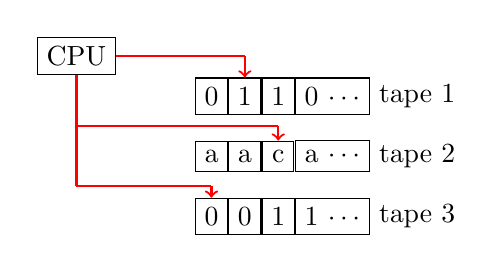
\begin{tikzpicture}[ampersand replacement=\&]
\matrix 
{
  \node[draw](0) {CPU}; \& [1cm]  \& \node(1){} ; \&\&\& \\
  \& \node[draw]{0}; \& \node[draw](a){1}; \& \node[draw]{1}; \& \node[draw]{0 $\cdots$};  \& \node{tape 1};\\
\node(2){} ; \&  \&  \& \node(21){} ; \&\& \\  
\& \node[draw]{a}; \& \node[draw]{a}; \& \node[draw](b){c}; \& \node[draw]{a $\cdots$}; \&  \node{tape 2}; \\
\node(3){} ; \& \node(31){} ; \&  \&  \&\& \\
\& \node[draw](c){0}; \& \node[draw]{0}; \& \node[draw]{1}; \& \node[draw]{1 $\cdots$}; \&  \node{tape 3}; \\
};

\draw [-,red,thick] (0) -- (1.center) ;
\draw [->,red,thick] (1.center) -- (a) ;
\draw [-,red,thick] (0) -- (2.center) ;
\draw [-,red,thick] (2.center) -- (21.center) ;
\draw [->,red,thick] (21.center) -- (b) ;
\draw [-,red,thick] (0) -- (3.center) ;
\draw [-,red,thick] (3.center) -- (31.center) ;
\draw [->,red,thick] (31.center) -- (c) ;
\end{tikzpicture}
\end{center}


\begin{center}
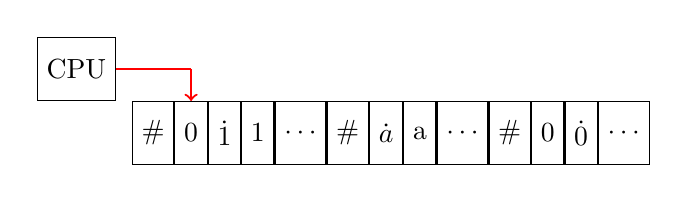
\begin{tikzpicture}[ampersand replacement=\&]
\matrix[nodes={minimum height=8mm}] 
{
  \node[draw](0) {CPU}; \& [0.2cm] \& \node(1){} ; \&\& \&\&\& \&\&\& \&\&\& \\
\& \node[draw]{\#};  \& \node[draw](a){0}; \& \node[draw]{$\dot{1}$}; \& \node[draw]{1}; \& \node[draw]{$\cdots$};
\& \node[draw]{\#};  \& \node[draw]{$\dot{\text{a}}$}; \& \node[draw]{a}; \& \node[draw]{$\cdots$}; 
\& \node[draw]{\#};  \& \node[draw](c){0}; \& \node[draw]{$\dot{0}$}; \& \node[draw]{$\cdots$}; \\
};

\draw [-,red,thick] (0) -- (1.center) ;
\draw [->,red,thick] (1.center) -- (a) ;
\end{tikzpicture}
\end{center}

  \begin{itemize}
\item
  \#: a symbol to separate tapes
\item $\dot{0}$ is used to store the head position of a tape
  
\item $\Gamma$ becomes different:

\item [] $\Gamma$ of original multi-tape TM:
  \begin{equation*}
  \{0,1,a,b,\ldots \}
\end{equation*}
\item [] $\Gamma$ of new single-tape TM:
  \begin{equation*}
  \{0,\dot{0},1,\dot{1},a,\dot{a},b,
\dot{b},\ldots \}
\end{equation*}
\item One multi-tape transition is split to several transitions
\item [] We sequentially conduct them
\item What if the transition is ``move to right (R)'' but we
  see \#?

\item [] $\Rightarrow$ insert a $\sqcup$ and shift things after
\item How to do the shift? An illustration:

  \begin{center}
\begin{tikzpicture}
  \node[state] (q_s) {$q_s$};
  \node[state,above right of=q_s,xshift=1.7cm] (q_0) {$q_0$};
  \node[state,below right of=q_s,xshift=1.7cm] (q_1) {$q_1$};
  \node[state,below right of=q_0,xshift=1.7cm] (q_a) {$q_a$};    
  \path (q_s) edge[above] node{
       $0 \rightarrow \sqcup,$ R
     } (q_0);
  \path (q_s) edge[below] node{
       $1 \rightarrow \sqcup,$ R
  } (q_1);
  \path (q_0) edge[bend right=15, left] node{
       $1 \rightarrow 0,$ R
     } (q_1);
  \path (q_0) edge[loop right] node{
       $0 \rightarrow $ R
  } (q_0);
  \path (q_1) edge[bend right=15, right] node{
       $0 \rightarrow 1,$ R
  } (q_0);
  \path (q_1) edge[loop right] node{
       $1 \rightarrow $ R
  } (q_1);
  \path (q_0) edge[above] node{
       $\sqcup \rightarrow 0$ 
  } (q_a);
  \path (q_1) edge[below] node{
       $\sqcup \rightarrow 1$ 
  } (q_a);
\end{tikzpicture}
  \end{center}

\item $\Gamma$ is finite. Use states to remember the current
  contents
\end{itemize}\end{frame}

\end{document}

%%% Local Variables:
%%% mode: latex
%%% TeX-master: t
%%% End:

